\documentclass[14pt]{extbook}
\usepackage{multicol, enumerate, enumitem, hyperref, color, soul, setspace, parskip, fancyhdr} %General Packages
\usepackage{amssymb, amsthm, amsmath, bbm, latexsym, units, mathtools} %Math Packages
\everymath{\displaystyle} %All math in Display Style
% Packages with additional options
\usepackage[headsep=0.5cm,headheight=12pt, left=1 in,right= 1 in,top= 1 in,bottom= 1 in]{geometry}
\usepackage[usenames,dvipsnames]{xcolor}
\usepackage{dashrule}  % Package to use the command below to create lines between items
\newcommand{\litem}[1]{\item#1\hspace*{-1cm}\rule{\textwidth}{0.4pt}}
\pagestyle{fancy}
\lhead{Makeup Progress Quiz -1}
\chead{}
\rhead{Version A}
\lfoot{7547-2949}
\cfoot{}
\rfoot{Fall 2020}
\begin{document}

\begin{enumerate}
\litem{
Solve the quadratic equation below. Then, choose the intervals that the solutions belong to, with $x_1 \leq x_2$ (if they exist).\[ -17x^{2} -7 x + 4 = 0 \]\begin{enumerate}[label=\Alph*.]
\item \( x_1 \in [-18.9, -16.7] \text{ and } x_2 \in [17.18, 17.91] \)
\item \( x_1 \in [-7.5, -4.1] \text{ and } x_2 \in [12.4, 12.88] \)
\item \( x_1 \in [-1.5, -0.4] \text{ and } x_2 \in [-0.14, 0.44] \)
\item \( x_1 \in [-0.6, 1] \text{ and } x_2 \in [0.66, 0.82] \)
\item \( \text{There are no Real solutions.} \)

\end{enumerate} }
\litem{
Graph the equation below.\[ f(x) = (x+4)^2 - 14 \]\begin{enumerate}[label=\Alph*.]
\begin{multicols}{2}\item 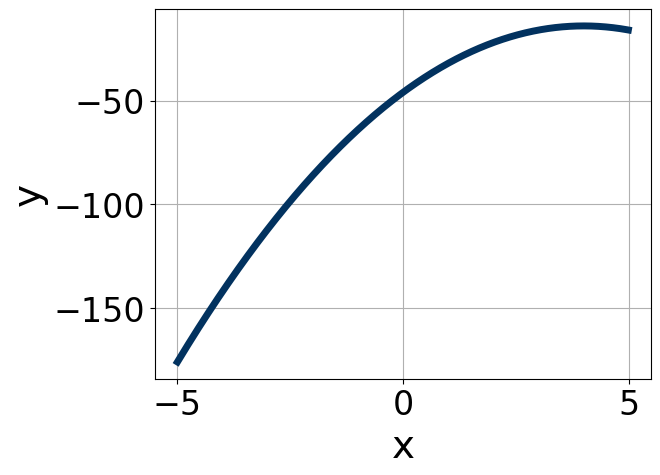
\includegraphics[width = 0.3\textwidth]{../Figures/quadraticEquationToGraphCopyAA.png}\item 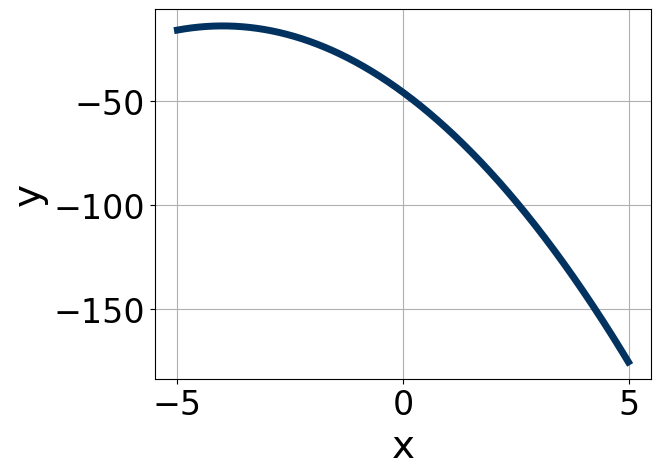
\includegraphics[width = 0.3\textwidth]{../Figures/quadraticEquationToGraphCopyBA.png}\item 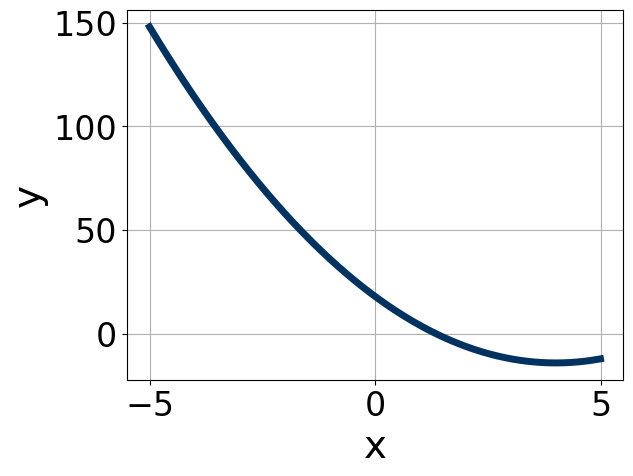
\includegraphics[width = 0.3\textwidth]{../Figures/quadraticEquationToGraphCopyCA.png}\item 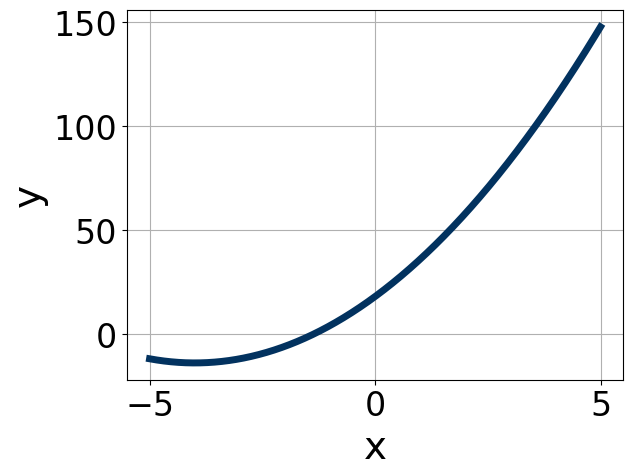
\includegraphics[width = 0.3\textwidth]{../Figures/quadraticEquationToGraphCopyDA.png}\end{multicols}\item None of the above.
\end{enumerate} }
\litem{
Graph the equation below.\[ f(x) = -(x-4)^2 + 12 \]\begin{enumerate}[label=\Alph*.]
\begin{multicols}{2}\item 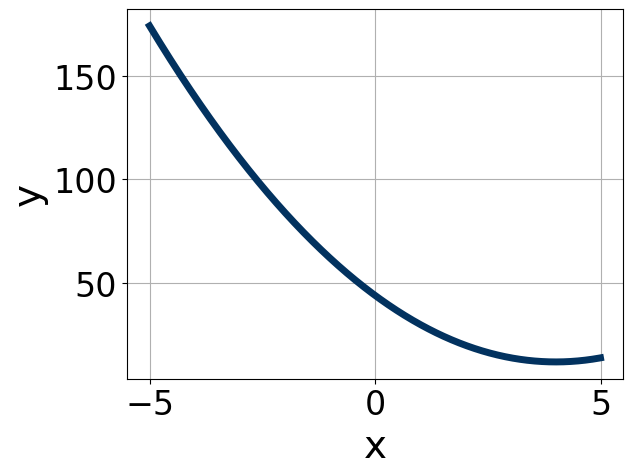
\includegraphics[width = 0.3\textwidth]{../Figures/quadraticEquationToGraphAA.png}\item 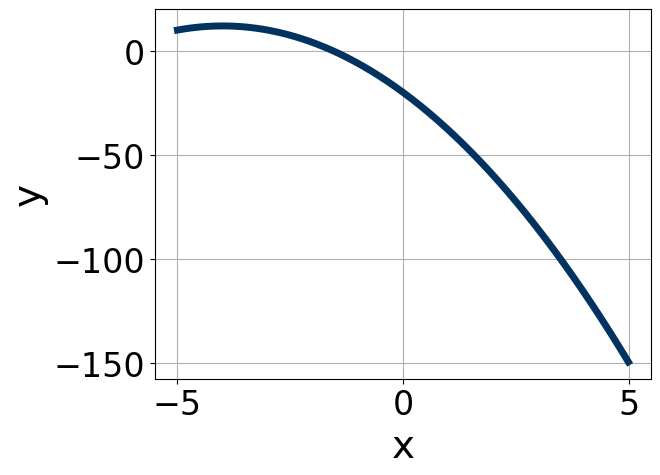
\includegraphics[width = 0.3\textwidth]{../Figures/quadraticEquationToGraphBA.png}\item 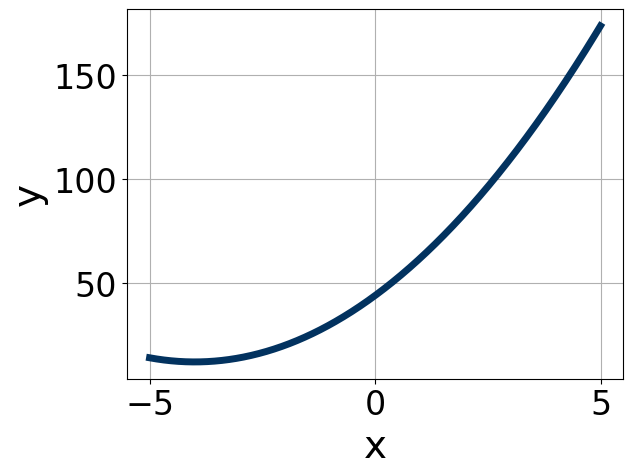
\includegraphics[width = 0.3\textwidth]{../Figures/quadraticEquationToGraphCA.png}\item 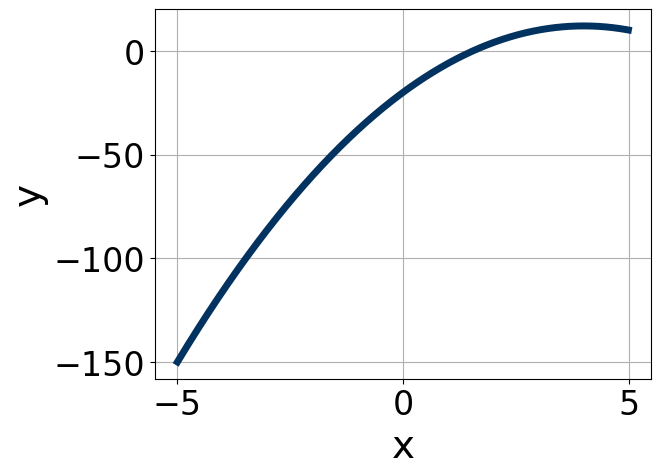
\includegraphics[width = 0.3\textwidth]{../Figures/quadraticEquationToGraphDA.png}\end{multicols}\item None of the above.
\end{enumerate} }
\litem{
Solve the quadratic equation below. Then, choose the intervals that the solutions $x_1$ and $x_2$ belong to, with $x_1 \leq x_2$.\[ 10x^{2} -63 x + 81 = 0 \]\begin{enumerate}[label=\Alph*.]
\item \( x_1 \in [0.88, 0.98] \text{ and } x_2 \in [8.4, 10.3] \)
\item \( x_1 \in [1.78, 1.95] \text{ and } x_2 \in [-0.7, 5] \)
\item \( x_1 \in [17.88, 18.09] \text{ and } x_2 \in [43.2, 47.5] \)
\item \( x_1 \in [0.54, 0.64] \text{ and } x_2 \in [11.3, 14.9] \)
\item \( x_1 \in [1.47, 1.54] \text{ and } x_2 \in [4.7, 5.6] \)

\end{enumerate} }
\litem{
Write the equation of the graph presented below in the form $f(x)=ax^2+bx+c$, assuming  $a=1$ or $a=-1$. Then, choose the intervals that $a, b,$ and $c$ belong to.
\begin{center}
    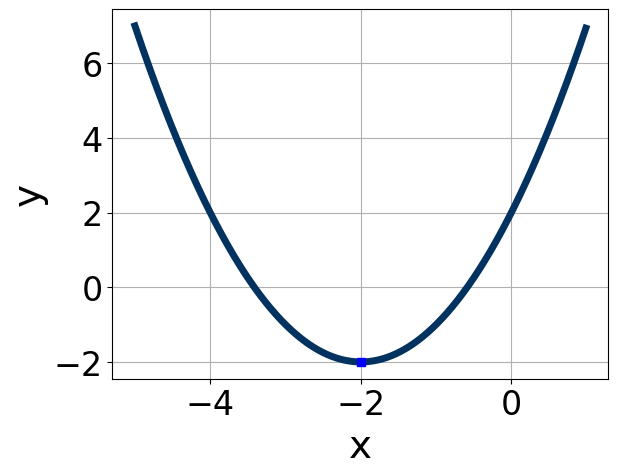
\includegraphics[width=0.5\textwidth]{../Figures/quadraticGraphToEquationCopyA.png}
\end{center}
\begin{enumerate}[label=\Alph*.]
\item \( a \in [1, 2], \hspace*{5mm} b \in [-4, -2], \text{ and } \hspace*{5mm} c \in [2, 4] \)
\item \( a \in [1, 2], \hspace*{5mm} b \in [-4, -2], \text{ and } \hspace*{5mm} c \in [5, 7] \)
\item \( a \in [-4, 0], \hspace*{5mm} b \in [3, 6], \text{ and } \hspace*{5mm} c \in [-7, -3] \)
\item \( a \in [1, 2], \hspace*{5mm} b \in [3, 6], \text{ and } \hspace*{5mm} c \in [2, 4] \)
\item \( a \in [-4, 0], \hspace*{5mm} b \in [-4, -2], \text{ and } \hspace*{5mm} c \in [-7, -3] \)

\end{enumerate} }
\litem{
Factor the quadratic below. Then, choose the intervals that contain the constants in the form $(ax+b)(cx+d); b \leq d.$\[ 54x^{2} -21 x -20 \]\begin{enumerate}[label=\Alph*.]
\item \( a \in [15.87, 18.8], \hspace*{5mm} b \in [-7, 2], \hspace*{5mm} c \in [1.8, 5.3], \text{ and } \hspace*{5mm} d \in [2, 8] \)
\item \( a \in [0.55, 1.3], \hspace*{5mm} b \in [-45, -40], \hspace*{5mm} c \in [-2.9, 1.1], \text{ and } \hspace*{5mm} d \in [21, 29] \)
\item \( a \in [1.45, 2.22], \hspace*{5mm} b \in [-7, 2], \hspace*{5mm} c \in [25.6, 27.6], \text{ and } \hspace*{5mm} d \in [2, 8] \)
\item \( a \in [4.61, 7.05], \hspace*{5mm} b \in [-7, 2], \hspace*{5mm} c \in [7.6, 12.9], \text{ and } \hspace*{5mm} d \in [2, 8] \)
\item \( \text{None of the above.} \)

\end{enumerate} }
\litem{
Solve the quadratic equation below. Then, choose the intervals that the solutions $x_1$ and $x_2$ belong to, with $x_1 \leq x_2$.\[ 10x^{2} -57 x + 54 = 0 \]\begin{enumerate}[label=\Alph*.]
\item \( x_1 \in [0.39, 0.69] \text{ and } x_2 \in [7.93, 9.23] \)
\item \( x_1 \in [1.31, 1.63] \text{ and } x_2 \in [3.19, 3.63] \)
\item \( x_1 \in [0.87, 0.97] \text{ and } x_2 \in [5.9, 6.02] \)
\item \( x_1 \in [0.93, 1.26] \text{ and } x_2 \in [4.17, 4.51] \)
\item \( x_1 \in [11.87, 12.39] \text{ and } x_2 \in [44.71, 45.36] \)

\end{enumerate} }
\litem{
Factor the quadratic below. Then, choose the intervals that contain the constants in the form $(ax+b)(cx+d); b \leq d.$\[ 36x^{2} +60 x + 25 \]\begin{enumerate}[label=\Alph*.]
\item \( a \in [2.9, 3.9], \hspace*{5mm} b \in [3, 6], \hspace*{5mm} c \in [9.3, 13.4], \text{ and } \hspace*{5mm} d \in [2, 11] \)
\item \( a \in [5.2, 7.6], \hspace*{5mm} b \in [3, 6], \hspace*{5mm} c \in [5.4, 6.6], \text{ and } \hspace*{5mm} d \in [2, 11] \)
\item \( a \in [-1.4, 2.8], \hspace*{5mm} b \in [26, 31], \hspace*{5mm} c \in [0.2, 1.7], \text{ and } \hspace*{5mm} d \in [29, 32] \)
\item \( a \in [11.9, 13.1], \hspace*{5mm} b \in [3, 6], \hspace*{5mm} c \in [1.2, 5.9], \text{ and } \hspace*{5mm} d \in [2, 11] \)
\item \( \text{None of the above.} \)

\end{enumerate} }
\litem{
Solve the quadratic equation below. Then, choose the intervals that the solutions belong to, with $x_1 \leq x_2$ (if they exist).\[ 19x^{2} -8 x -4 = 0 \]\begin{enumerate}[label=\Alph*.]
\item \( x_1 \in [-0.53, 0.41] \text{ and } x_2 \in [0.51, 1.25] \)
\item \( x_1 \in [-2.33, -0.65] \text{ and } x_2 \in [-0.2, 0.6] \)
\item \( x_1 \in [-19.55, -18.55] \text{ and } x_2 \in [18.06, 19.85] \)
\item \( x_1 \in [-6.09, -4.74] \text{ and } x_2 \in [12.77, 14.98] \)
\item \( \text{There are no Real solutions.} \)

\end{enumerate} }
\litem{
Write the equation of the graph presented below in the form $f(x)=ax^2+bx+c$, assuming  $a=1$ or $a=-1$. Then, choose the intervals that $a, b,$ and $c$ belong to.
\begin{center}
    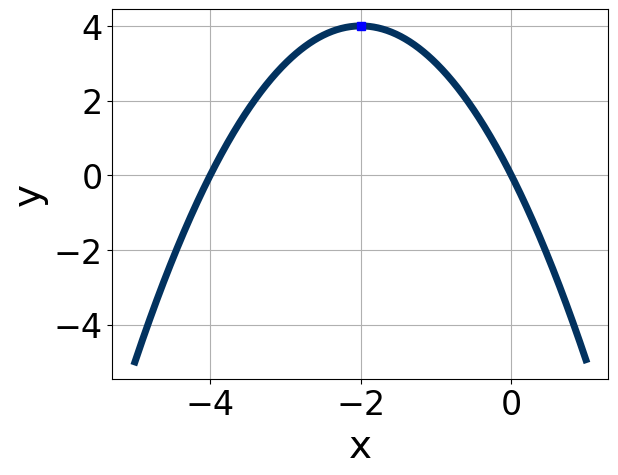
\includegraphics[width=0.5\textwidth]{../Figures/quadraticGraphToEquationA.png}
\end{center}
\begin{enumerate}[label=\Alph*.]
\item \( a \in [0.9, 3], \hspace*{5mm} b \in [-4, -1], \text{ and } \hspace*{5mm} c \in [6, 10] \)
\item \( a \in [-1.6, 0.7], \hspace*{5mm} b \in [3, 5], \text{ and } \hspace*{5mm} c \in [0, 1] \)
\item \( a \in [-1.6, 0.7], \hspace*{5mm} b \in [3, 5], \text{ and } \hspace*{5mm} c \in [-8, -7] \)
\item \( a \in [-1.6, 0.7], \hspace*{5mm} b \in [-4, -1], \text{ and } \hspace*{5mm} c \in [0, 1] \)
\item \( a \in [0.9, 3], \hspace*{5mm} b \in [3, 5], \text{ and } \hspace*{5mm} c \in [6, 10] \)

\end{enumerate} }
\end{enumerate}

\end{document}